\section{商业模式设计}

商业模式设计方法有:\textbf{客户洞察}、\textbf{构思}、\textbf{视觉化思考}、\textbf{模型构建}、\textbf{讲故事}和\textbf{场景}。

\subsection{客户洞察}

客户视角是商业模式设计的指导性原则。客户的观点决定了我们选择怎样的价值主张、渠道、客户关系和收益来源。

企业一般都会在市场研究上投入重金,但它们最终设计产品、服务和商业模式的时候往往又会忽略客户的观点。要想设计好的商业模式,必须避免这类错误
\begin{itemize}
    \item 必须通过客户的眼睛来观察商业模式,这样就有可能发现全新的机会。
    \item 难点在于对客户透彻的理解。商业模式的设计必须基于这份理解。在产品和服务设计领域,很多业界领先的企业都通过与社会学家一起合作来加深他们的理解。
    \item 创新的真正挑战在于深入理解客户,而不是简单地去问他们要什么。
    \begin{itemize}
        \item  汽车工业的先驱亨利·福特曾经说过:“要是我去问客户他们想要什么,他们会要一匹更快的马。”
    \end{itemize}
    \item 另一个难点在于企业是否清楚需要关注哪些客户、忽略哪些客户。
    \begin{itemize}
        \item 在很多情况下,能够拉动未来增长的那些客户往往并不是今天的金牛客户。
        \item 商业模式的创新不能仅仅聚焦现有的客户群体,必须着眼于新客户群体。
    \end{itemize}
\end{itemize}

\subsubsection{移情图}
\begin{figure}[H]
	\centering
	\vspace{-0.5em}
	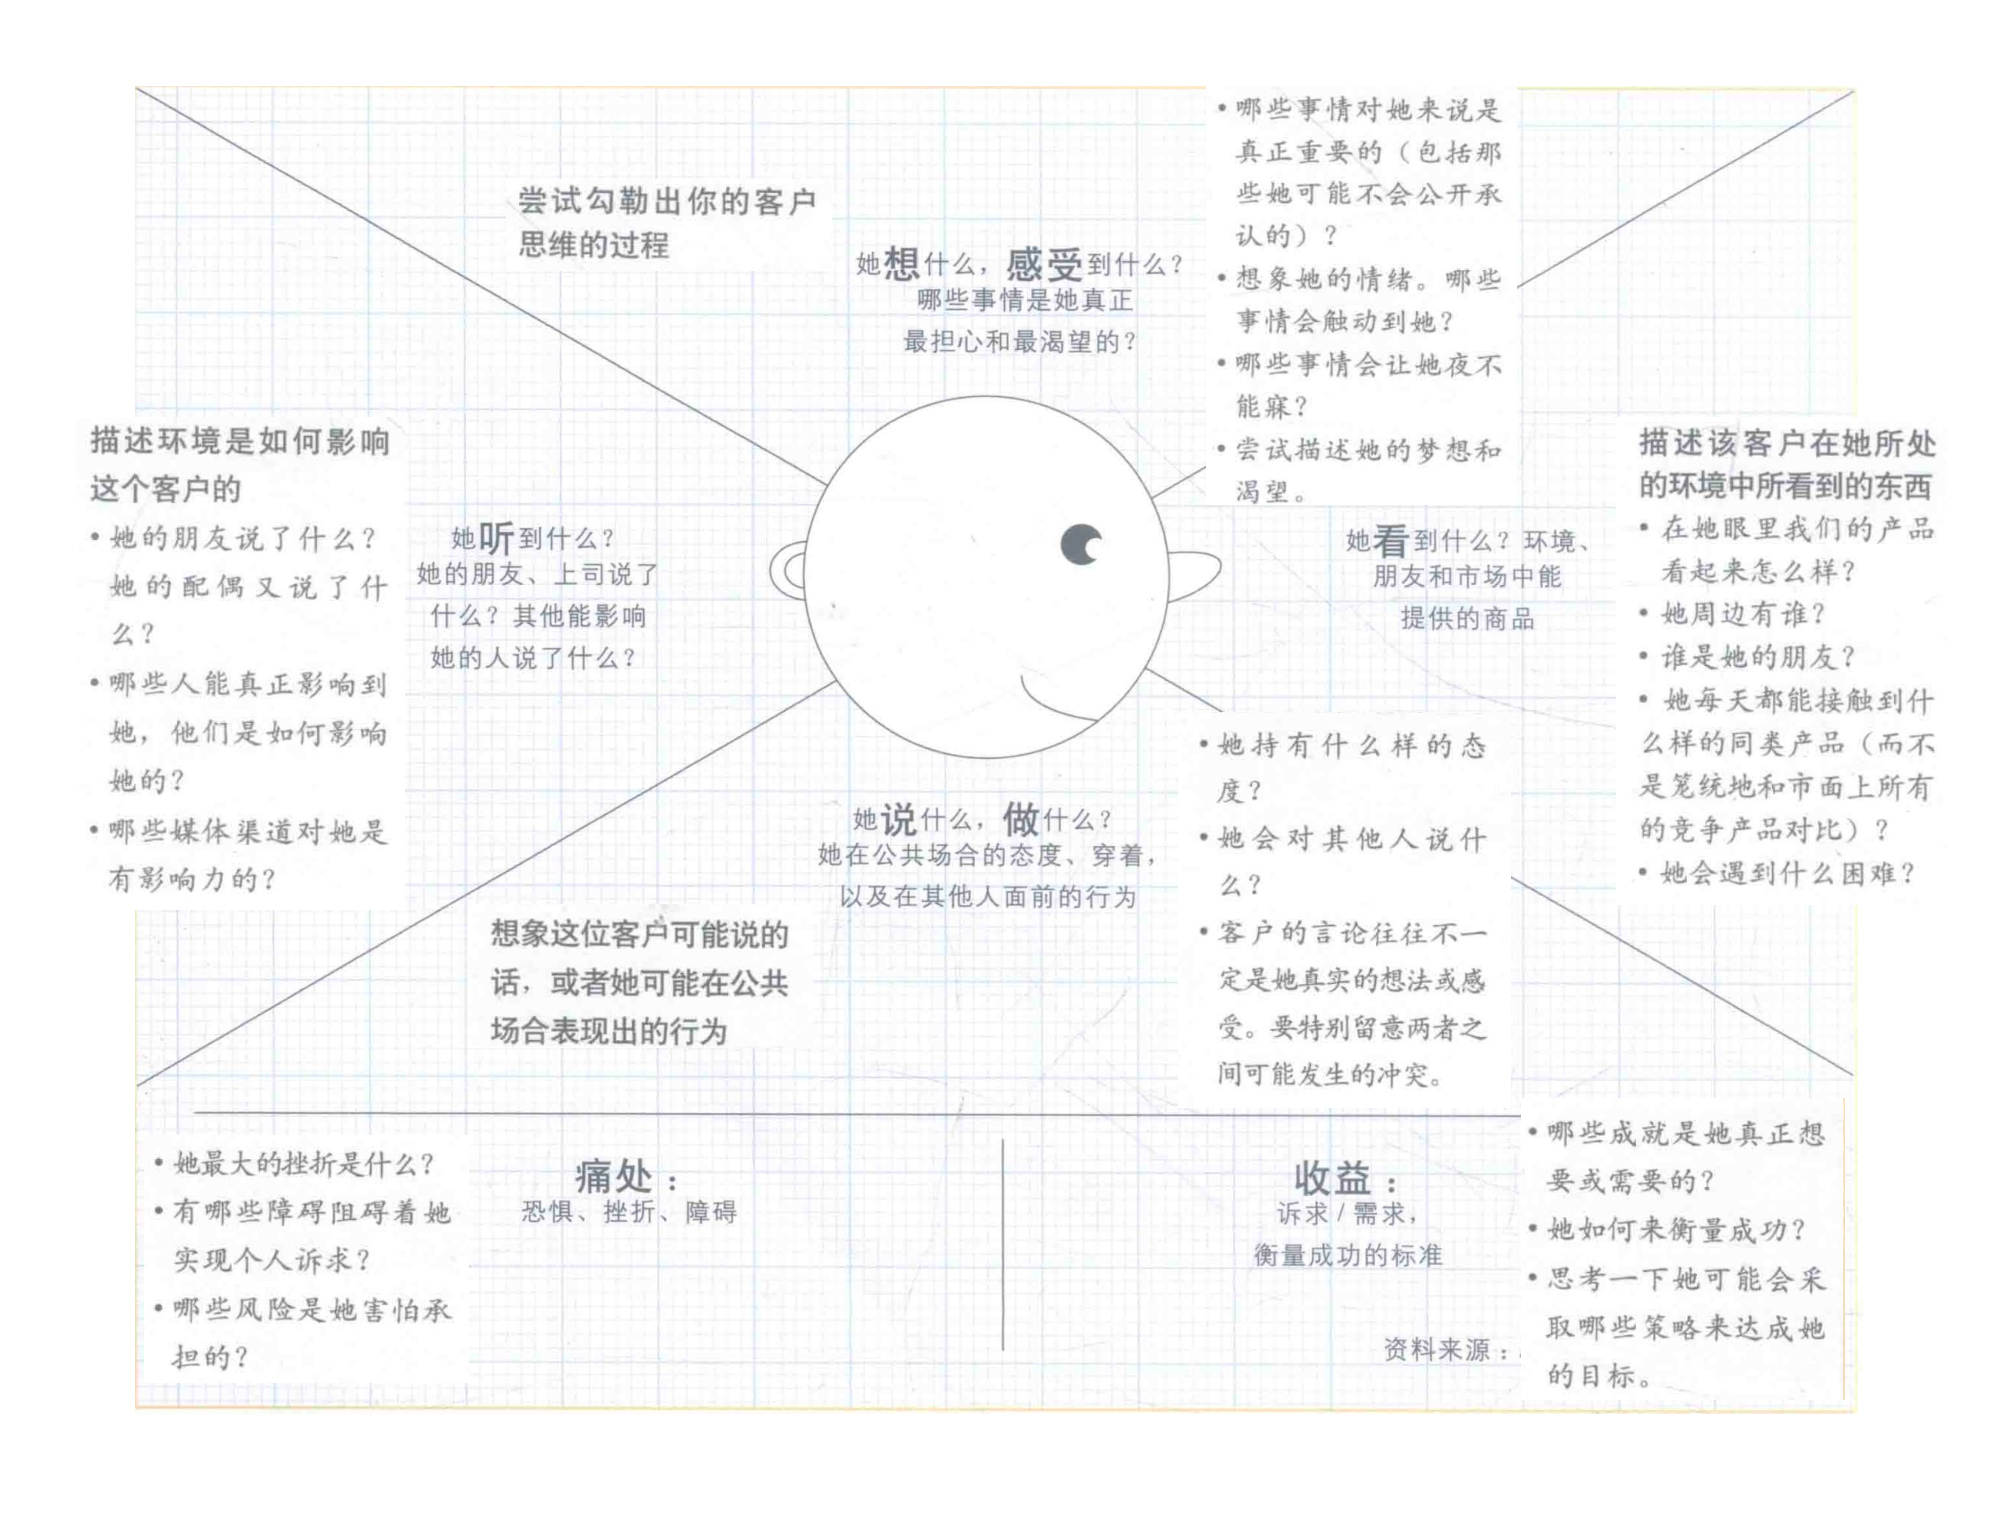
\includegraphics[width=0.95\textwidth]{img/移情图.pdf}
    \vspace{-1em}
\end{figure}

移情图示例:微软在线Office产品对于目标企业的首席信息官CIO

\begin{figure}[H]
	\centering
	\vspace{-0.5em}
	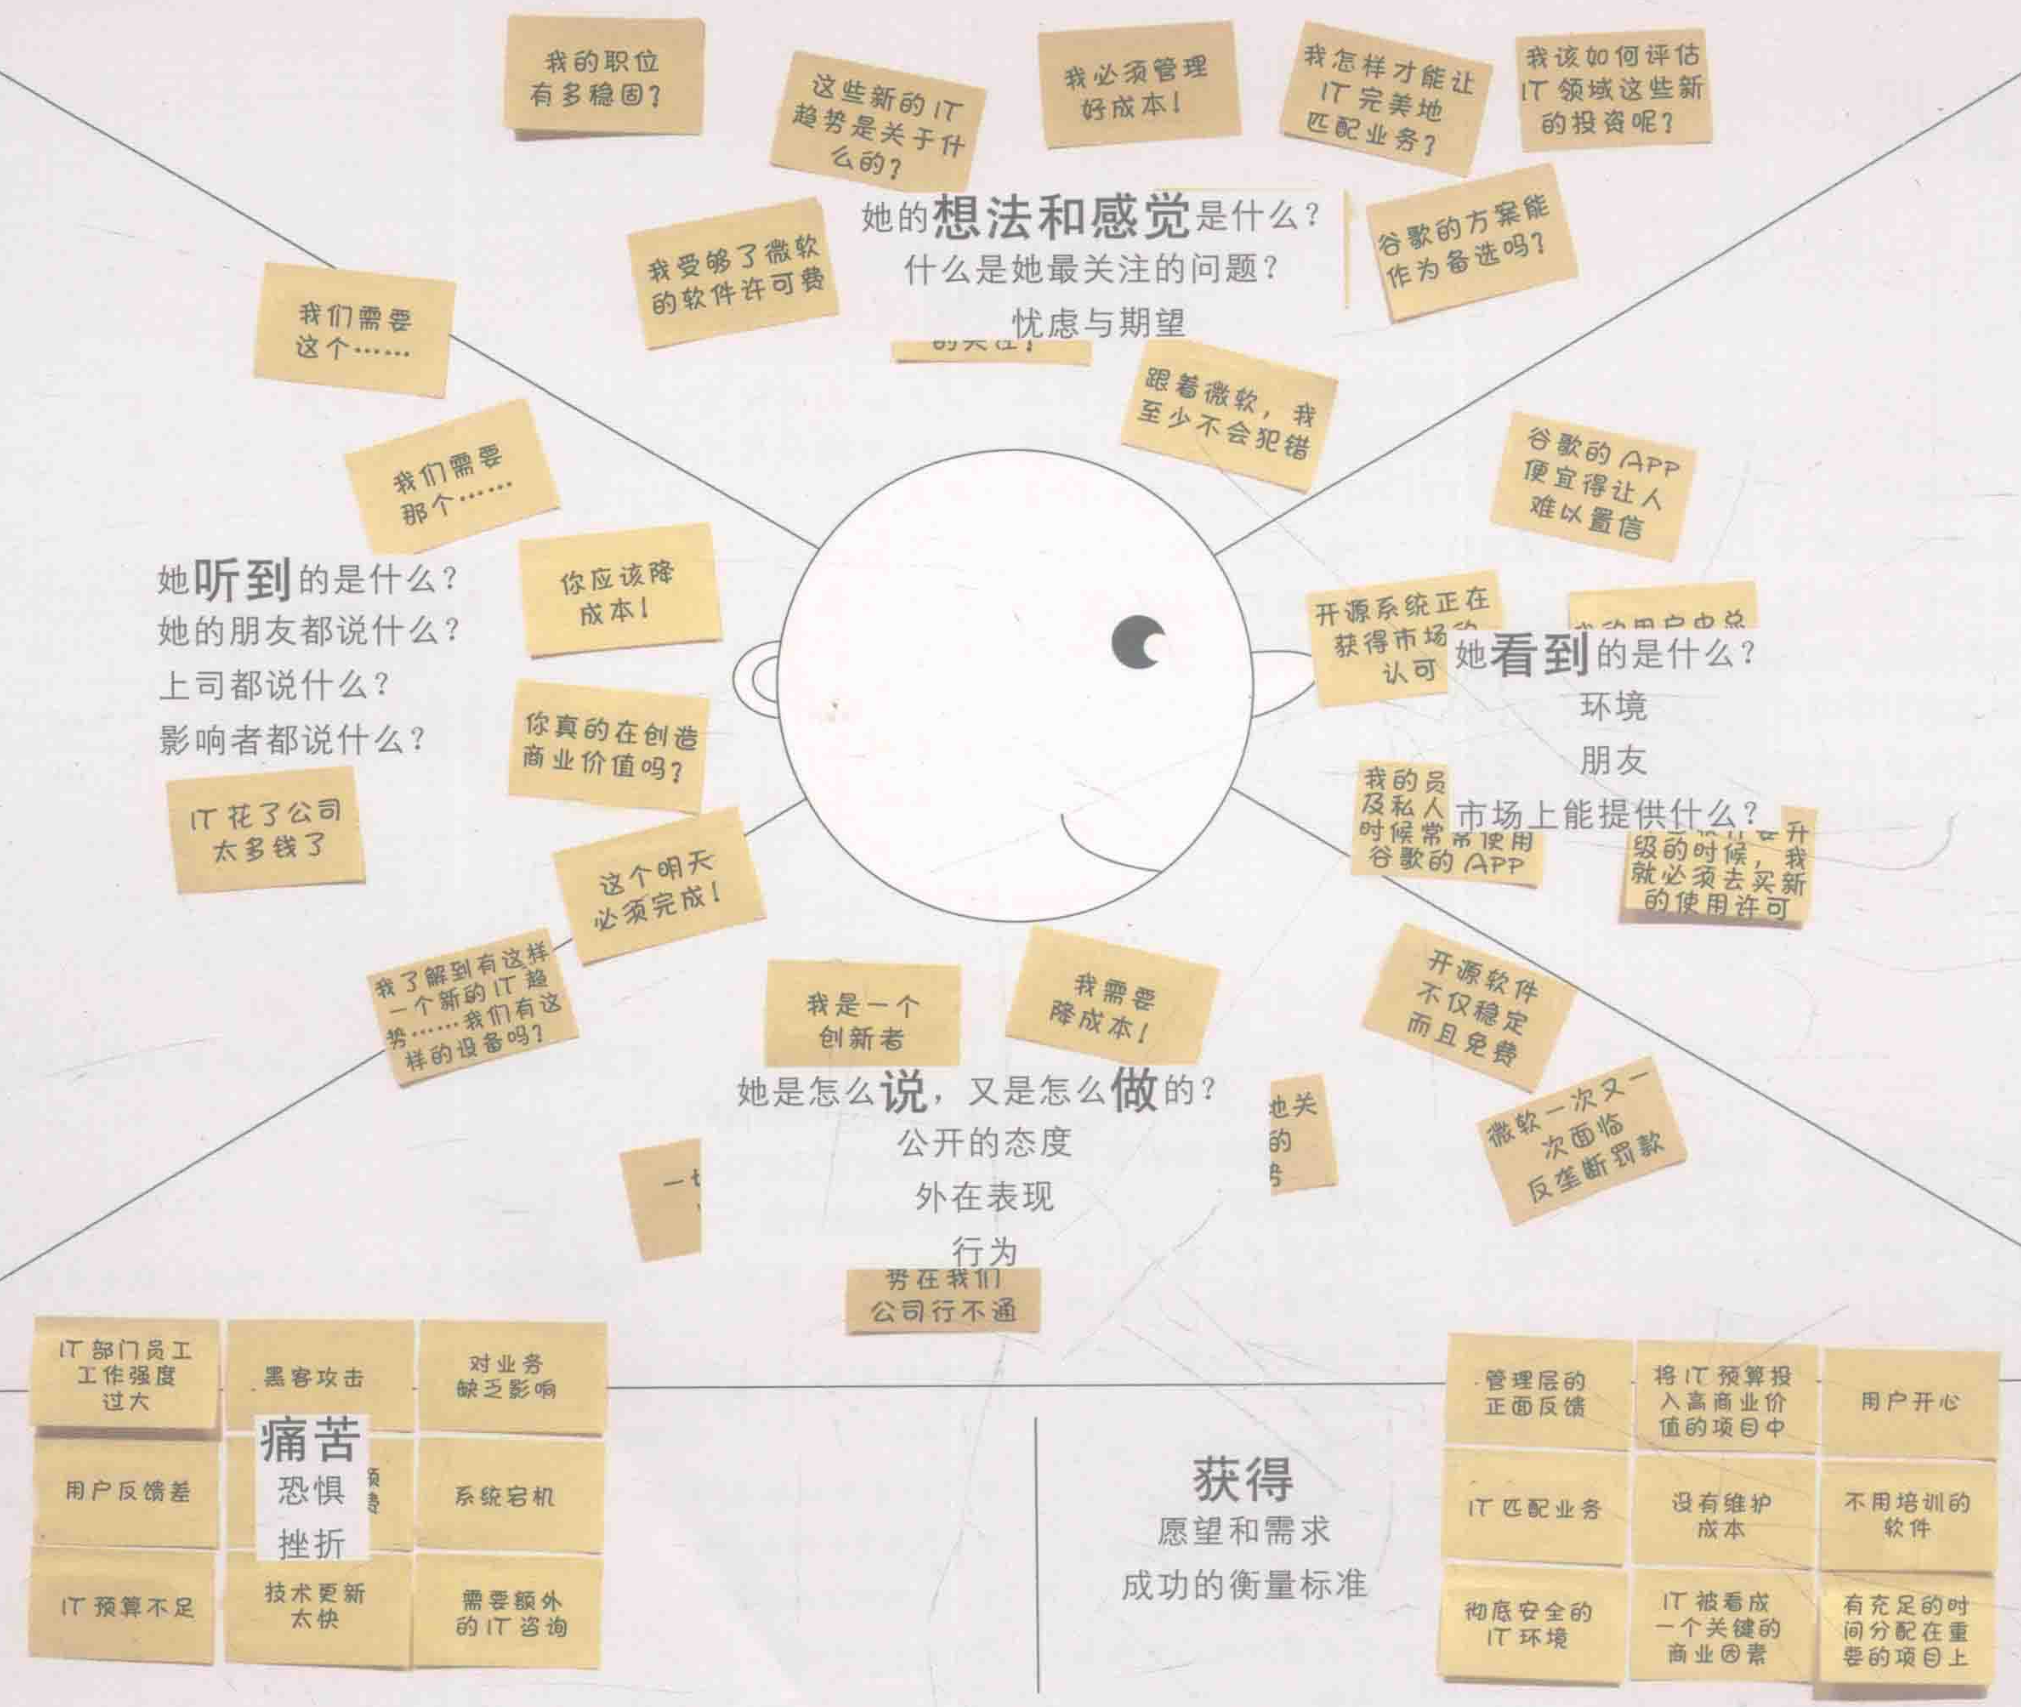
\includegraphics[width=0.8\textwidth]{img/移情图示例.png}
    \vspace{-0.5em}
\end{figure}


\subsection{构思}

通过一个创造性的流程来产生大量的商业模式创意,并且能成功地识别出最佳的创意。这个流程就被称为构思。
\begin{itemize}
    \item 构思的过程有两个主要阶段:
    \begin{itemize}
        \item 生成创意,这个阶段数量是重点
        \item 整合创意,这个阶段要把创意进行讨论、合并组合并甄选出少数可行的创意
    \end{itemize}
    \item 可行的创意并不一定要是颠覆性的商业模式。它们也可以是通过扩展你当前商业模式的领域来提升你的竞争力,这也是一种创新。
    \item 关注两点:在商业模式画布中你的商业模式创新的焦点和“如果……会怎样”的问题。
\end{itemize}

\subsubsection{商业模式创新的焦点}
\begin{itemize}
    \item 商业模式创新如果按照创新的焦点来分类,大致有4种:资源驱动、供给驱动、客户驱动和财务驱动。
    \item 这4个焦点中任何一个都可以作为重大商业模式变革的起点,也都有力地影响商业模式九宫格中的其他8个模块。
    \item 有些时候,商业模式创新可能会源自多个焦点。
    \item SWOT分析不失为一个好的工具来帮助我们找到变革的起点,它能够帮助企业深入解剖某个南业模式的优势、劣势、机会和威胁。
\end{itemize}

\begin{figure}[H]
	\centering
	\vspace{-0.5em}
	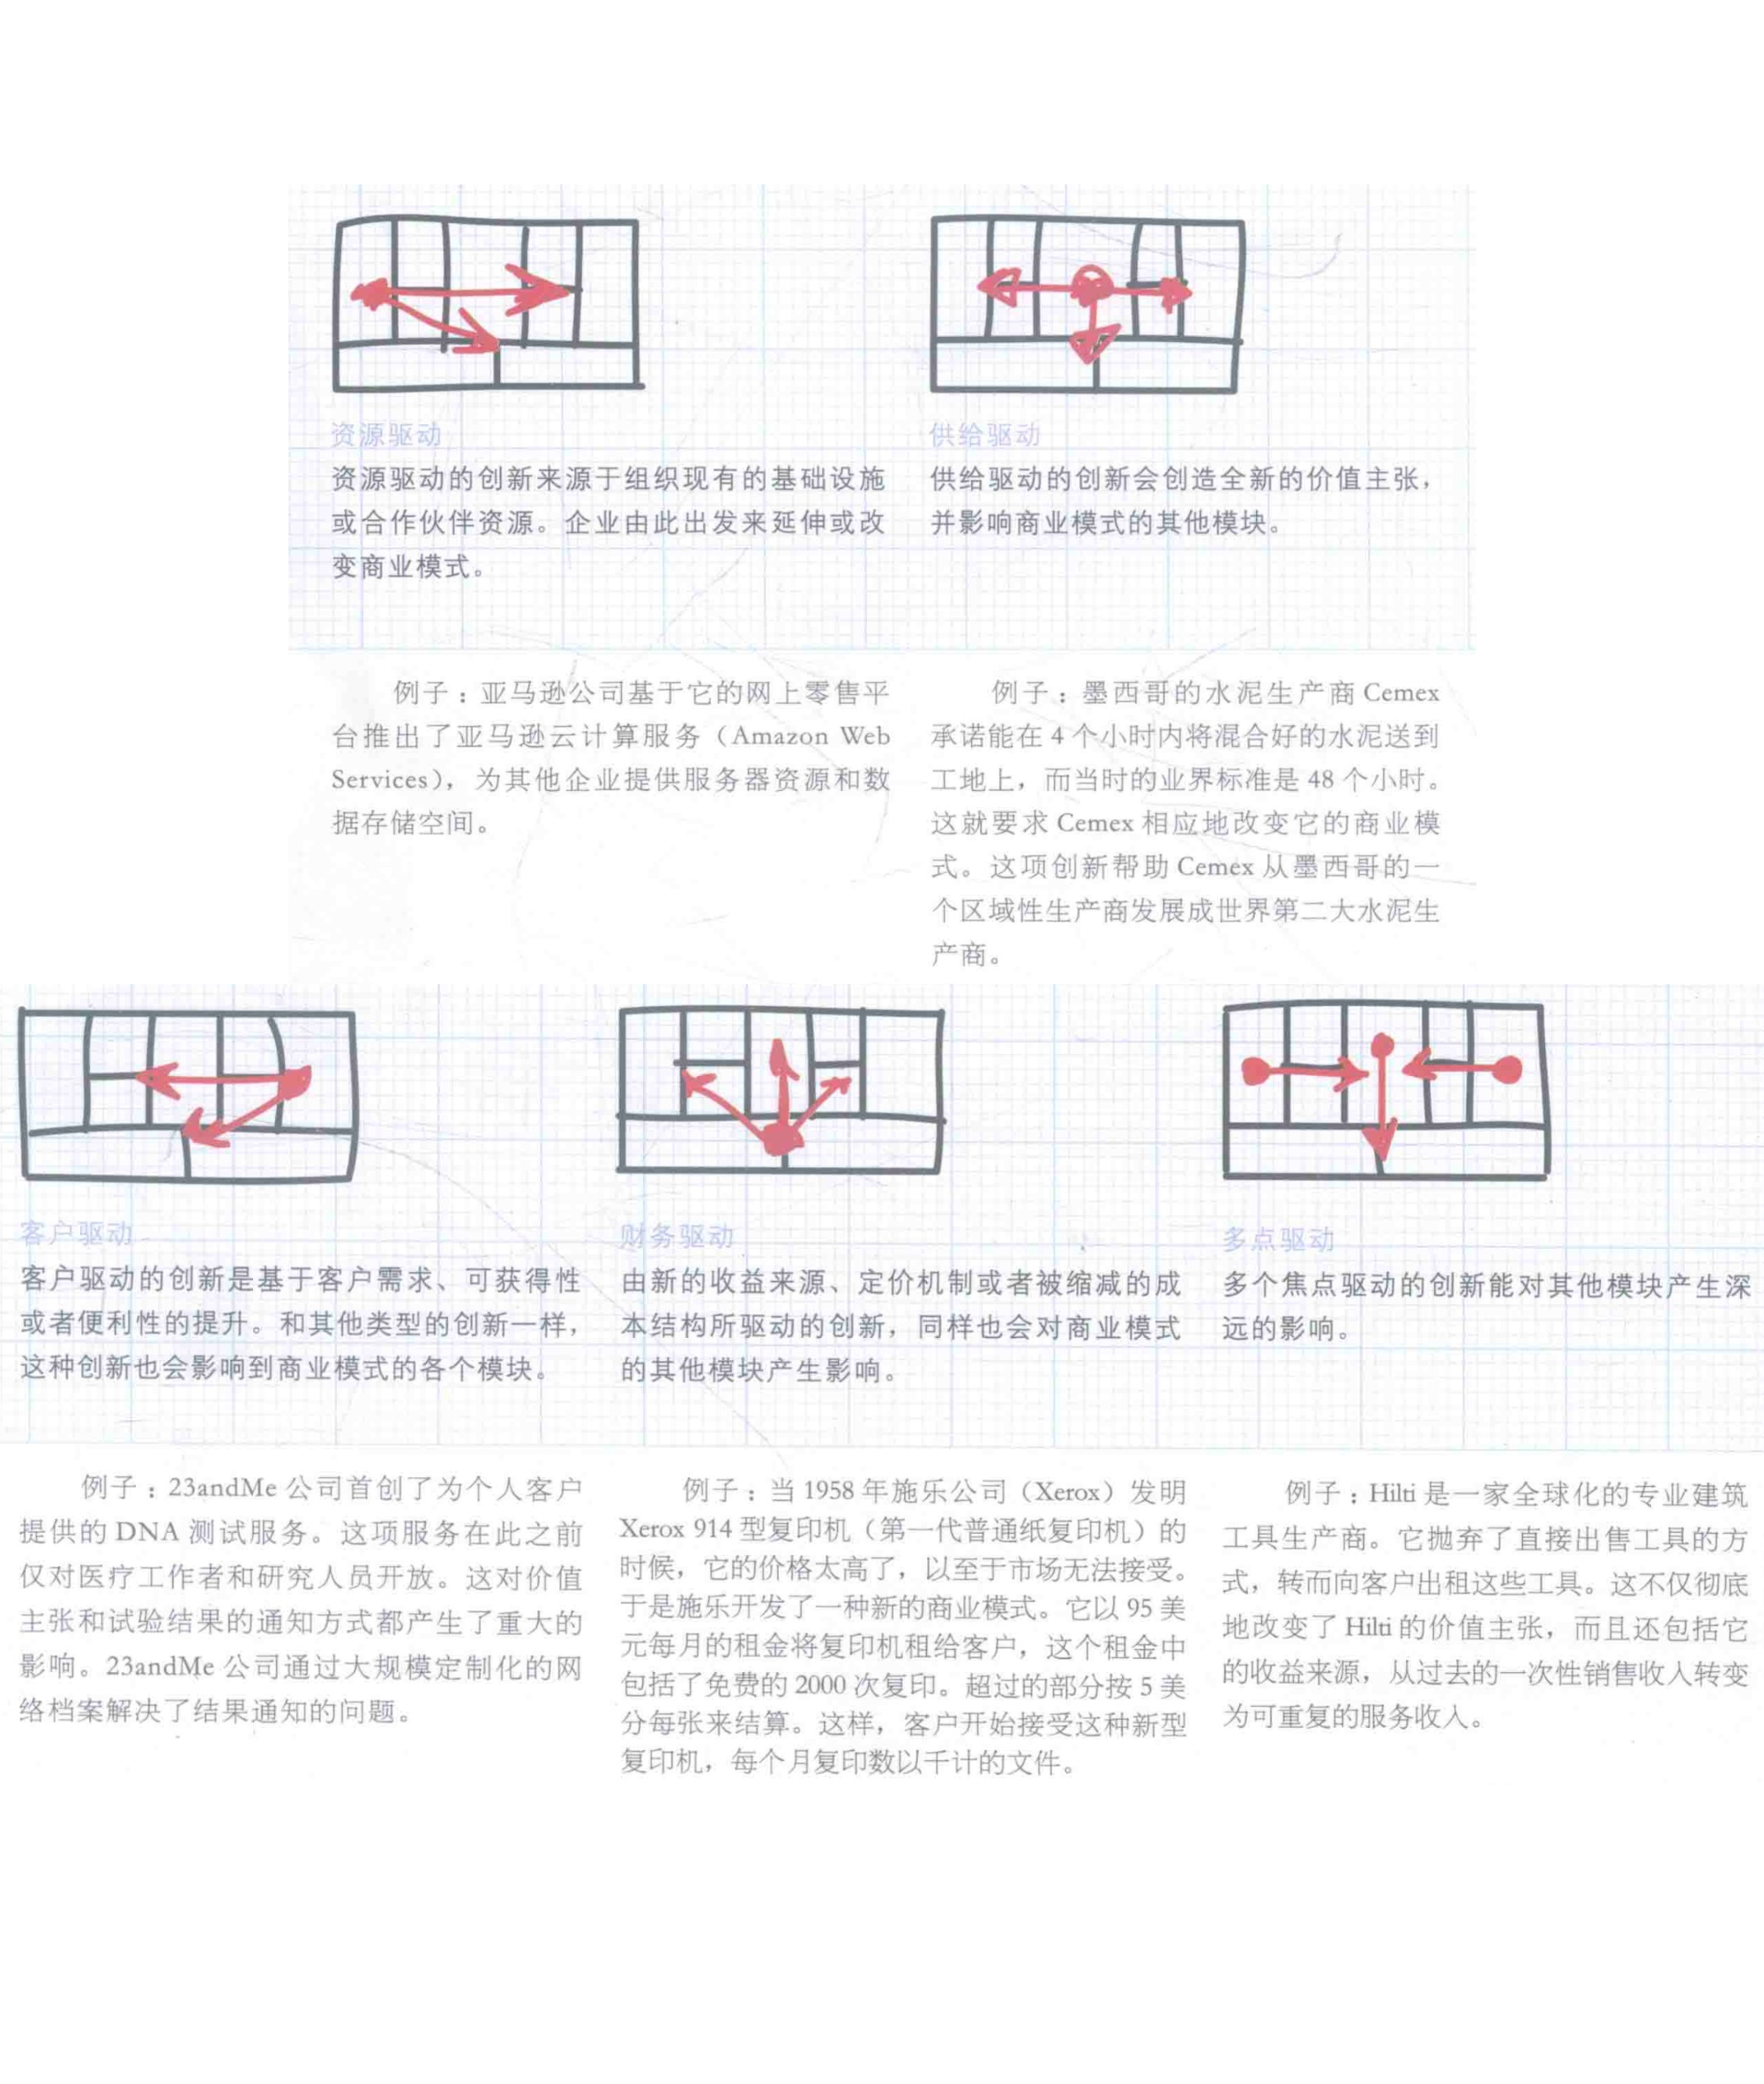
\includegraphics[width=0.9\textwidth]{img/商业模式创新的焦点.pdf}
    \vspace{-0.5em}
\end{figure}

\subsubsection{问题“如果……会怎样”的魔力}

受制于现状对思维的束缚,我们常常会苦于无法构思出创新的商业模式,现状遏制了想象力。
\begin{itemize}
    \item 克服这一问题的一个方法就是用“如果……会怎样”的问题来挑战传统假设。
    \item 有了正确的商业模式原料,一些原本认为不可能的事情也可以成为能够做到的事情。
    \item “如果……会怎样”的问题帮助我们挣脱现有商业模式的束缚。它们能激发我们,挑战我们的思维。它们还能让更多新奇的、难于执行的主张闯入我们的思维。
\end{itemize}

\subsubsection{构思的流程}
构思的流程可以采取很多种形式。这里给出的是一个能产生创新商业模式的总体方法:
\begin{enumerate}[label=\arabic*.]
    \item 团队组建:为了产生新颖的商业模式创意,我们的团队是否足够多样化?
    
    组建正确的团队对产生有效的新商业模式创意至关重要。团队成员的资历、年龄、经验水平、业务领域、客户知识和专业技能都要多样化。
    \item 钻研:在生成商业模式创意之前,我们必须钻研哪些知识?
    
    理想的团队必须经过钻研的阶段。这可能会包括总体研究、研究客户或潜在客户、详细调查新技术和评估现有的商业模式。钻研的过程可能会长达数周或短至一两次工具分析(比如移情图)。
    \item 开拓:我们能针对商业模式的每个模块做哪些创新?
    
    在这个阶段,团队尽可能地开拓解决方案的范围,以产生尽可能多的创意。商业模式九个模块中的任何一个都可以作为创新的起点。这个阶段的目的是数量,而非质量。使用头脑风暴的组织原则能让人们聚焦发掘创意,避免过早地评论创意的价值。
    \item 甄选标准:我们为商业模式创意排序最重要的标准是什么?
    
    在从最大范围上开拓了足能多的解决方案后,团队必须确定一个标准来从海量的创意中挑出数量在可管理范围内的少数创意。这个标准必须针对你的业务背景,同时还要涵盖诸如下内容:预期实施时间、潜在收入,可能的客户阻力和对竞争优势的影响。
    \item 构建模型:对于每一个进入短名单的创意,它完整的商业模式会是怎样的?
    
    标准一旦确立,团队必须有能力从若干创意中整理出一个最优创意的短名单,由此来构建$3\sim 5$个创新的商业模式。然后使用商业模式画布来勾勒和讨论每个商业模式模型。
\end{enumerate}

\subsubsection{组建一个多样化的团队}

\begin{itemize}
    \item 商业模式创新不应该仅仅限于研发或战略规划部门。
    \item 商业模式创新团队必须拥有多样化背景的团队成员。这种多样化会有助于你创造、讨论和甄选新的创意。你也可以添加一些外部人士,甚至儿童也是可以的。
    \item 多样化是有好处的。但你一定要保证能教会他们如何积极地倾听,并且考虑在关键会议上引入一个中立的引导员。
\end{itemize}

\subsubsection{头脑风暴的规则}

\begin{itemize}
    \item 保持聚焦:首先要精确地表达当前的问题。在理想情况下,这必须和客户需求有关。不要让讨论跑题太远,始终将讨论拉回到开始的问题上来。
    \item 执行规则:在一开始就闸明头脑风暴的规则并且坚决执行。其中最重要的规则是“不要过早下结论”、“每次一个人讲,不要七嘴八舌”、“追求数量”、“视觉化”和“鼓励疯狂的创意”。引导员必须执行好这些规则。
    \item 视觉化思考:把创意写下来或者画在每个人都能看到的地方。有一个搜集创意的好办法是把它们写在便利贴上, 然后贴到一面墙上。这样你可以随意地移动这些创意并将它们重新组合。
    \item 准备:通过对当前问题进行钻研来为头脑风暴做好准备。这些钻研活动可以是团队的一次实地考察以及与客户的讨论等任何形式的对你的问题陈述的钻研活动。
\end{itemize}


\subsection{视觉化思考}

\subsubsection{视觉化思考的价值}

\begin{itemize}
    \item 商业模式其实是一个内部元素相互影响的整体系统;它只有在形成一个整体的时候才是有意义的。不将它视觉化很难一目了然地抓住它的主旨。
    \item 视觉化能够一目了然的刻画商业模式的主旨,并具象化其中的隐含假设。
    \item 视觉化能够使商业模式变的明确,为团队讨论提供一些概念性的锚点,使讨论从抽象思维落实到具体、形象的东西。
    \item  视觉化既能找出已有模式中的逻辑缺陷,又能在设计全新模式时更容易地添加、删除和移动相关的图片化概念。
\end{itemize}

视觉化思考使用的两项技术与四个流程
\begin{itemize}
    \item 如何使用便利贴和如何将草图与商业模式画布结合
    \item 视觉化思考的四个流程:理解、对话、探索、沟通
\end{itemize}

\subsubsection{视觉化的实现:便利贴+绘画}
便利贴的重要性:可以随意地添加、移除,以及在商业模式各模块之间挪动
\begin{itemize}
    \item 三个简要的指导方针:用粗的马克笔、每张便利贴只写一项元素、每张便利贴上只用很少的字来抓住关键点
    \item 在用便利贴呈现的最终商业模式图景前的讨论过程和结果同样重要。参与者会讨论在画布上贴上哪张纸、移除哪张纸,辩论某项元素如何影响其他元素。
    \item 这些讨论过程都让参与者能深入地理解该商业模式和它的动态变化过程。最终,这些便利 贴就不仅仅代表了商业模式中的某个模块,它们引导了战略讨论的方向。   
\end{itemize}

绘画的强大表现力:人对图像的反应要比文字强烈的多
\begin{itemize}
    \item 最简陋的素描也能让事物变得具体和易于理解:如情绪、比例等。
    \item 帮助向别人解释和沟通你的商业模式,容易激发起建设性的讨论与创意。
    \item 可用于勾勒一个典型客户与他所处的环境,也可用于勾勒出客户群体的需求和任务。
\end{itemize}

\subsubsection{视觉化的作用}
\begin{itemize}
    \item 理解商业模式的本质
    \begin{itemize}
        \item 视觉化的语言:画布是一张概念图,其功能类似于具有语法规则的视觉化语言,提供了视觉和文字的指引,帮助画出模式中所需的所有信息
        \item 抓住全貌:画布的草图能够为观众提供足够的信息理解全貌,而不被过多的细节影响理解
        \item 看到关键:一定要理解元素/模块之间的关联关系
    \end{itemize}
    \item 提升对话效率
    \begin{itemize}
        \item 共同的参照点:将头脑中不言而喻的主观假设具象化,并将大量内容固化成为可回溯的参照点(人类的短时记忆只能保留有限数量的想法)
        \item 统一的语言:利用图形和画布帮助不同参与者聚焦,特别是来自不同领域的人
        \item 一致的理解:帮助不同部门的人将其深入理解的部分表达出来,再一起形成整体的洞察与一致的理解
    \end{itemize}
    \item 探索创意
    \begin{itemize}
        \item 激发创意:模糊的想法—随着灵感发挥—有机地整合成一幅图画
        \item 演习:视觉化的模型帮助思考部分元素的改变引发的系统性冲击
    \end{itemize}
    \item 提升沟通
    \begin{itemize}
        \item 统一公司内部的理解:用图画在组织内形成共识,朝一个战略方向前进
        \item 内部推销:好的图画使组织的现状、需要做的事情、怎么做、未来会怎样等方面变得易于沟通,从而赢得组织内部的理解和支撑
        \item 外部推销:提升向投资人或潜在合作伙伴推销成功的概率 
    \end{itemize}
\end{itemize}

\subsubsection{为不同的需求采取不同的视觉化方式}
根据目标的不同,视觉化的商业模式需要展示出不同程度的细节。例如Skype的商业模式就直观地展现了它与传统电信运营商的关键区别。它的目标在于指出Skype商业模式与传统运营商的显著差异,尽管它们提供类似的服务。

\begin{figure}[H]
	\centering
	\vspace{-0.5em}
	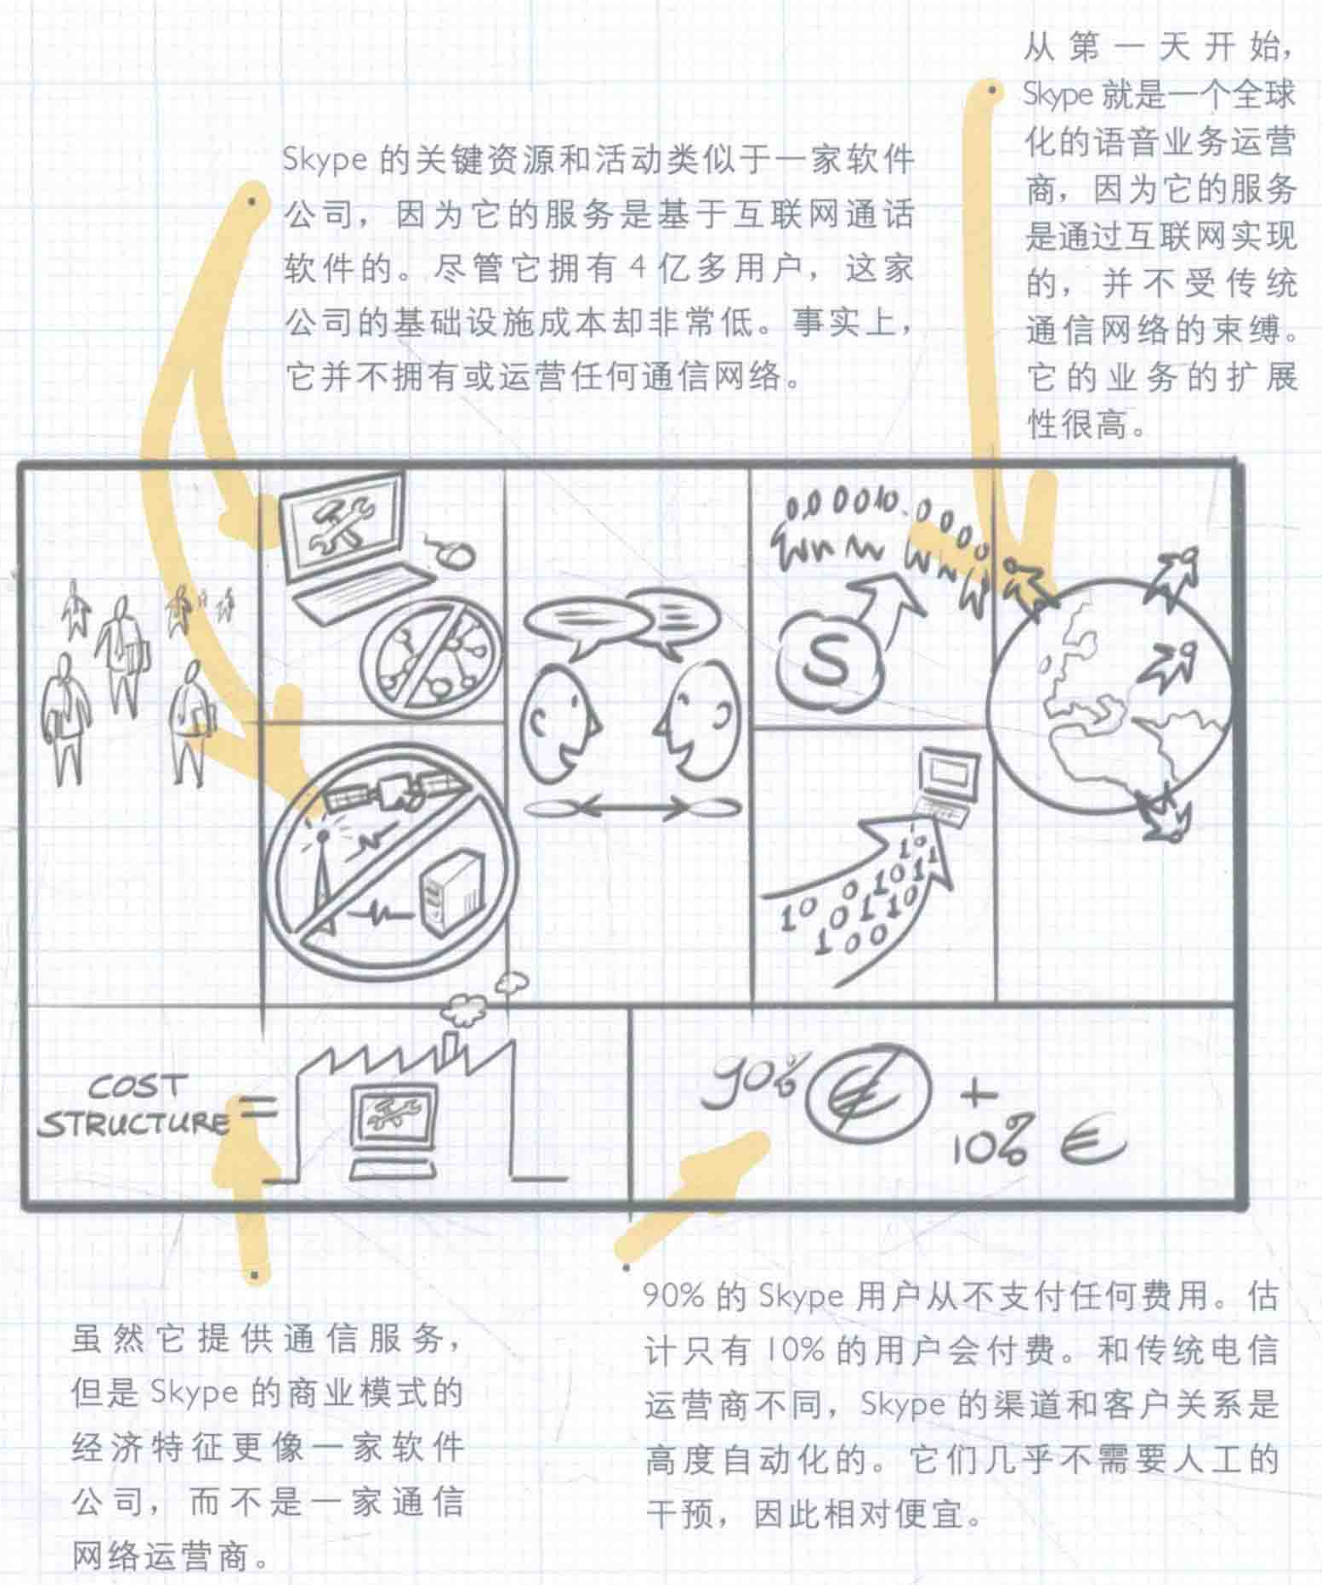
\includegraphics[width=0.6\textwidth]{img/为不同的需求采取不同的视觉化方式.png}
    \vspace{-0.5em}
\end{figure}

\subsubsection{讲述一个视觉化的故事}

解释商业模式的一种有力的方式:利用画布草图逐一介绍一个完整的视觉化故事

如何讲述视觉化故事
\begin{figure}[H]
	\centering
	\vspace{-0.5em}
	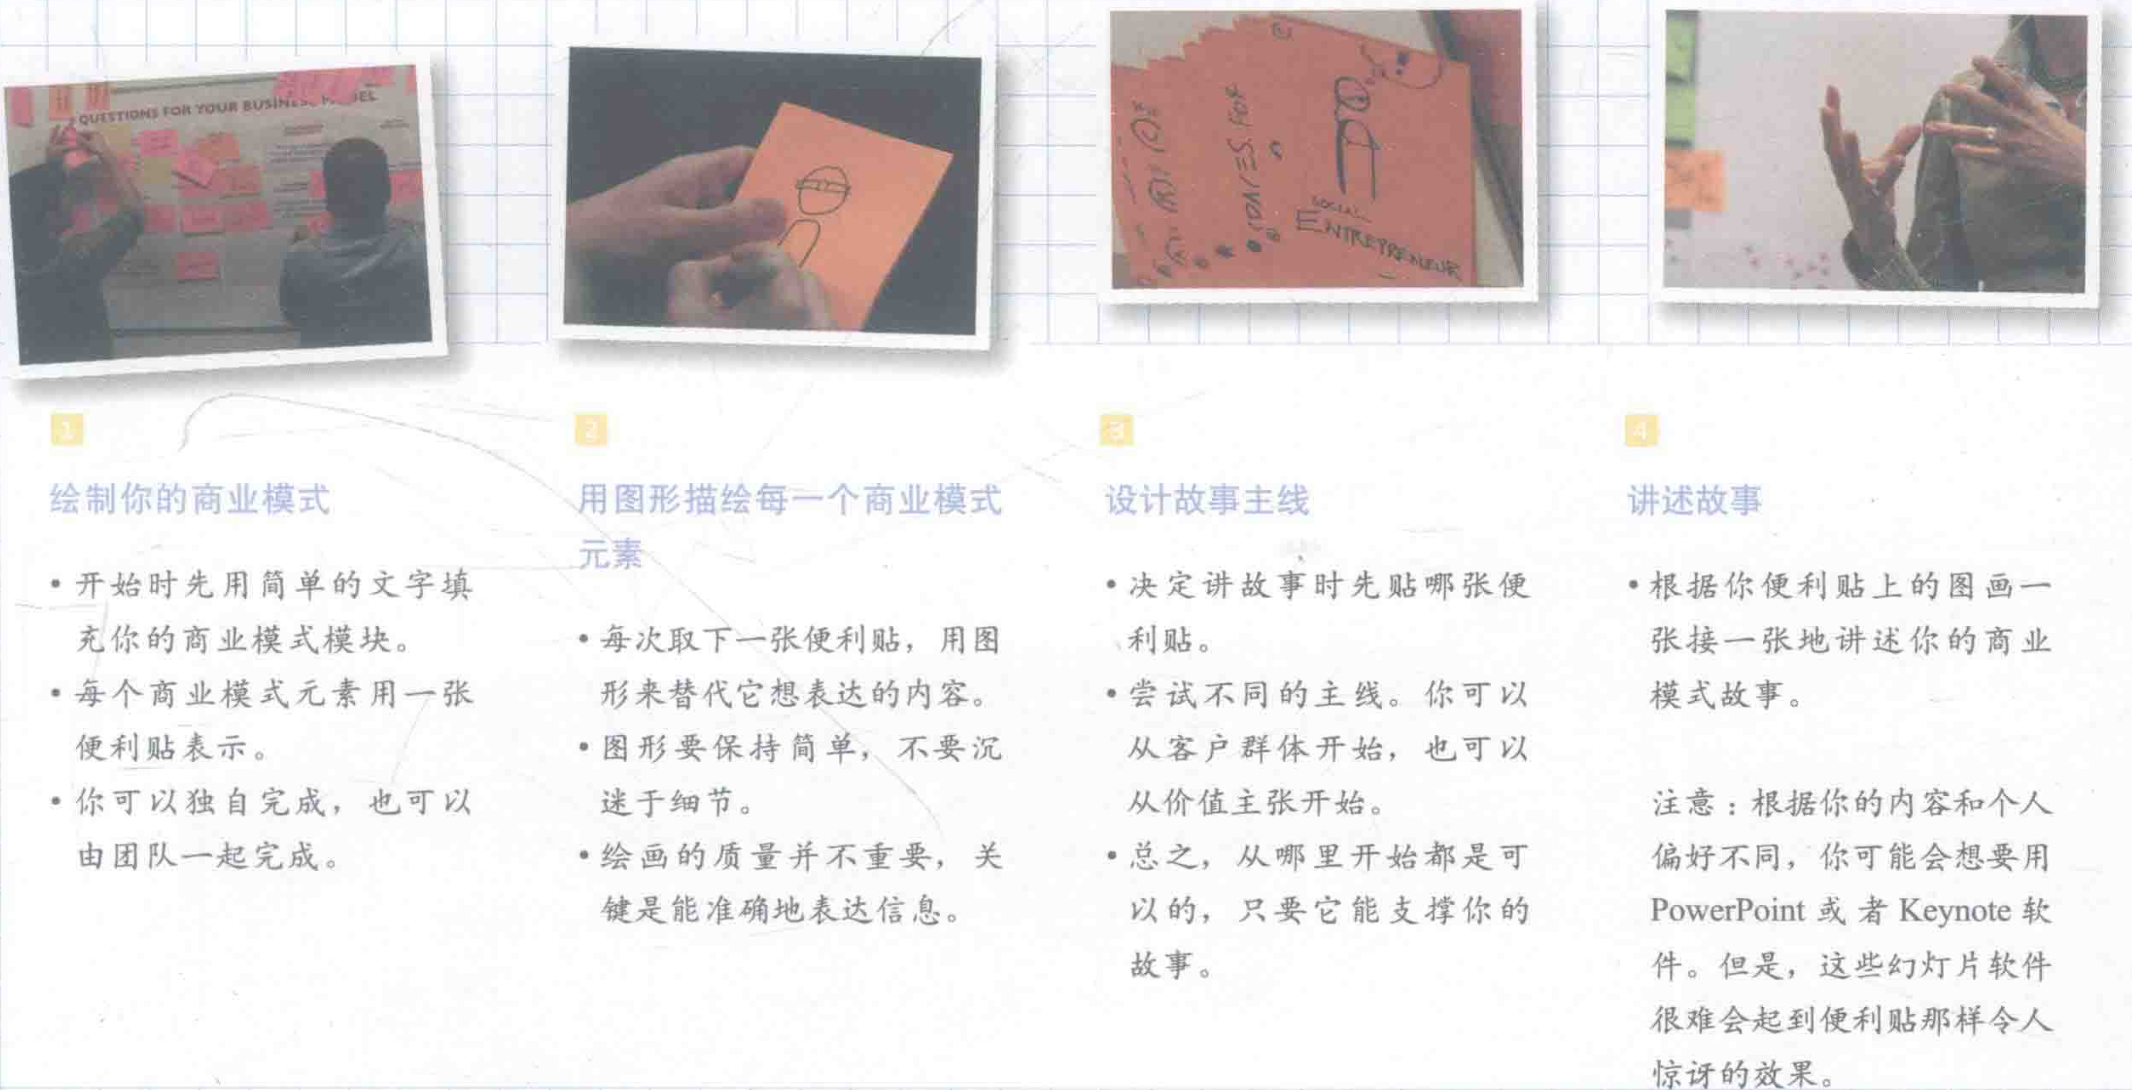
\includegraphics[width=0.9\textwidth]{img/如何讲述视觉化故事.png}
    \vspace{-0.5em}
\end{figure}

\subsection{模型构建}

\subsubsection{模型构建的价值}
模型构建是一个很有力的工具,可以开发出新颖、创新的商业模式。
\begin{itemize}
    \item 和视觉化思考一样,模型构建可以让抽象的概念具体化,有助于探索出新的创意。
    \begin{itemize}
        \item 模型构建这项技术来自设计学和工程学,被广泛地用在产品设计、架构设计和交互式设计。它在商业管理领域却不是很常用,主要是因为组织行为和战略的抽象性。
        \item 把模型看成未来潜在的商业模式:是一个用于讨论、探究或者概念验证的工具。
        \item 一个商业模式模型可以是一张简单的草图,一张充分思考过的商业模式画布,或者是一叠模拟新商业模式财务状况的数据表格。
    \end{itemize}
    \item 模型构建有助于实际商业模式的探索。
    \begin{itemize}
        \item 建模$\rightarrow$(疑问点明确化、视觉化)$\rightarrow$添加、删除或修改元素$\rightarrow$观察结果。
        \item 在不同规模(抽象层面)的模型上进行互动。
        \item 有助于获得突破性的商业模式,同时能够有效控制细节。
    \end{itemize}
\end{itemize}

\subsubsection{设计态度}
\begin{itemize}
    \item 设计态度包括了愿意去探素原始的想法,迅速地放弃这些想法,然后花时间检查多种可能性,直到选出少数值得优化的想法,而且要接受这种不确定性,直到设计方向成熟。
    \item 这些素质井不是专业人士与生俱来的,但它们是开发新的商业模式所必需的。
    \item 设计态度要求人们从做决定的思维转化为创造多种可选方案来选择的思维。
\end{itemize}

\subsubsection{构建不同规模的模型}
控制规模:通过绘制很多(粗略的和细致的)模型来代表各种战略选择,再通过对每个模型添加和移除元素的方式来探索新想法
\begin{itemize}
    \item 随手素描:勾勒和推销一个粗略的创意
    
    画一个简单的商业模式画布,仅仅用关键元素来描述这个创意
    \begin{itemize}
        \item 勾勒想法
        \item 包含价值主张
        \item 包含主要收益来源
    \end{itemize}
    \item 精心描绘的画布:探索实现该创意所需的因素
    
    通过描绘一个相对详细的面布来探索该商业模式所需的所有元素。
    \begin{itemize}
        \item 描绘整张画布
        \item 通过你的商业逻辑来思考
        \item 预估市场潜力
        \item 理解商业模式画布各个模块之间的关系
        \item 做一些基本的“事实查证”工作
    \end{itemize}
    \item 商业案例:检查该创意的可存活度
    
    将详细的画布转化为财务表格,估算你的商业模式的盈利潜力
    \begin{itemize}
        \item 建立一张全面的画布
        \item 包含关键数据
        \item 计算成本和收入
        \item 估算利润潜力
        \item 根据不同的假设进行财务场景模拟
    \end{itemize}

    \item 实地验证:调查用户的接受度和可行性
    
    你已经在一个潜在的新商业模式上下定决心,现在需要去实地验证它的某个方面。
    \begin{itemize}
        \item 为这个新商业模式准备一个合情合理的商业案例
        \item 站在客户的角度或者让真实的客户来进行实地验证
        \item 验证价值主张、渠道、定价机制等实际市场中的元素
    \end{itemize}
\end{itemize}

利用模型构建探究决策到执行的转换
\begin{figure}[H]
	\centering
	\vspace{-0.5em}
	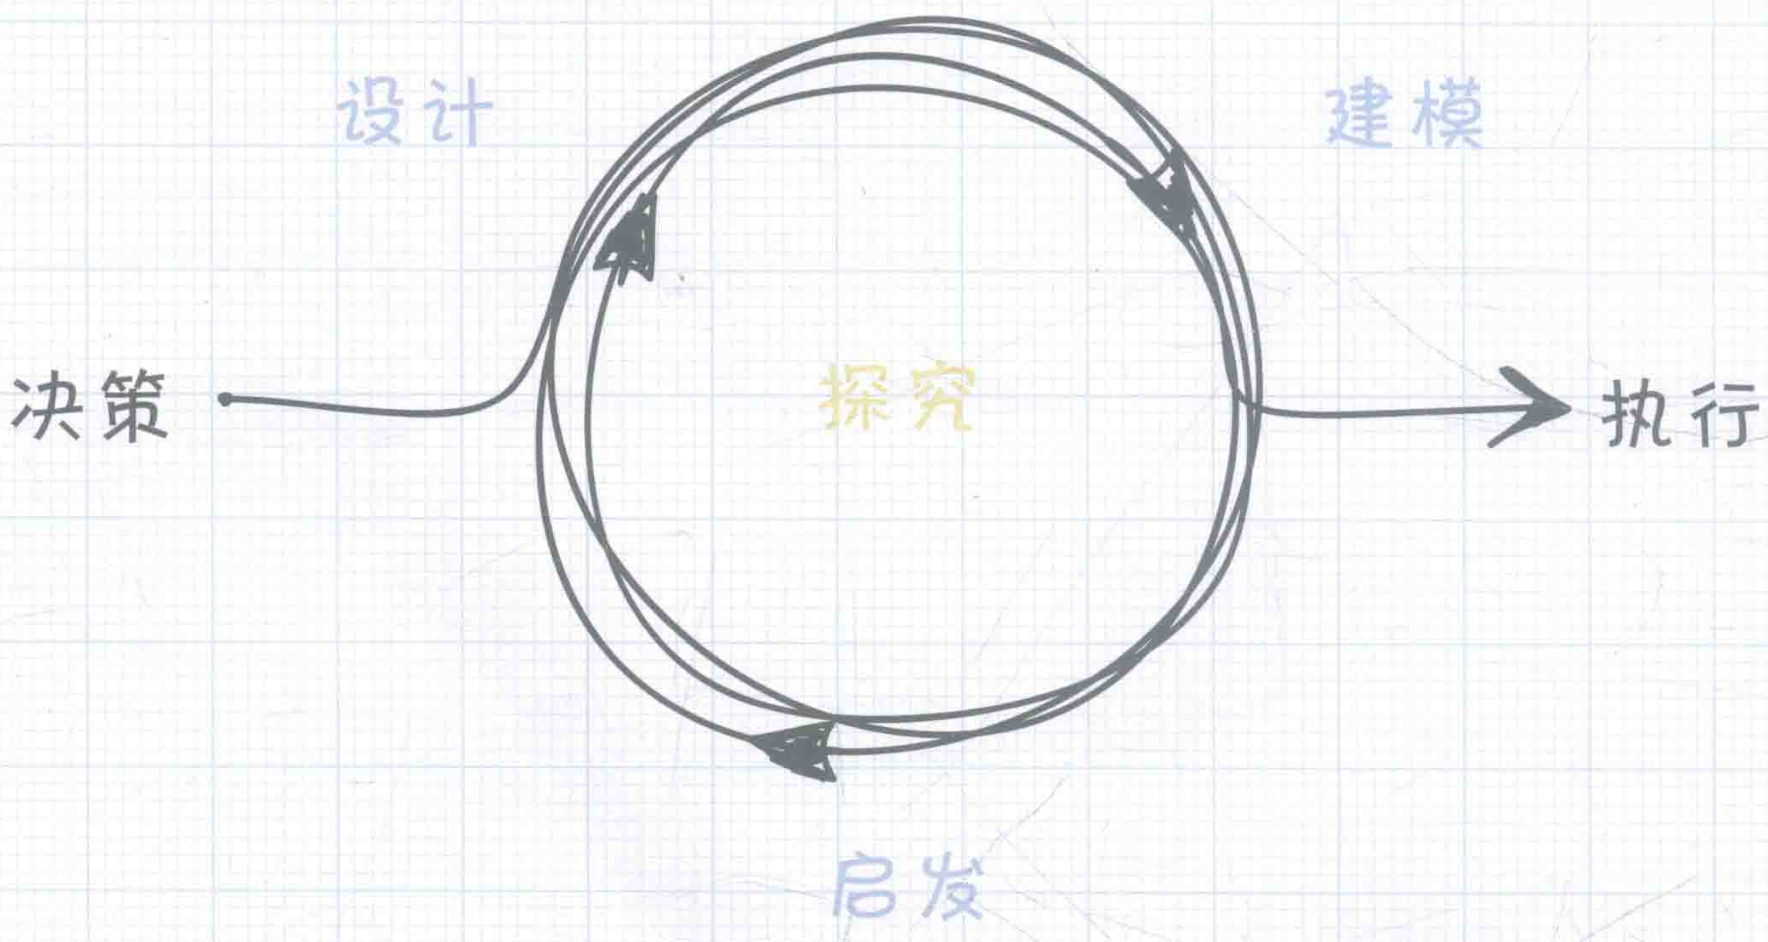
\includegraphics[width=0.5\textwidth]{img/利用模型构建探究决策到执行的转换.png}
    \vspace{-0.5em}
\end{figure}


\subsection{讲故事}

\subsubsection{讲故事的价值}
故事是一个理想的热身工具,为深度讨论商业模式与其内在逻辑做好准备
\begin{itemize}
    \item 将故事与画布结合,利用叙事性克服听众对不熟悉模式的抵触,放下对陌生事物的怀疑
\end{itemize}

为什么要讲故事
\begin{itemize}
    \item 介绍新想法:尝试融入组织战略
    \item 向投资人推销:争取外部资源
    \item 吸引员工:抓住组员的注意力和好奇心,为下一步探讨准备
    \item 让未来触手可及:激发创意、辩证变革
\end{itemize}

\subsubsection{故事的不同视角}
\begin{figure}[H]
	\centering
	\vspace{-0.5em}
	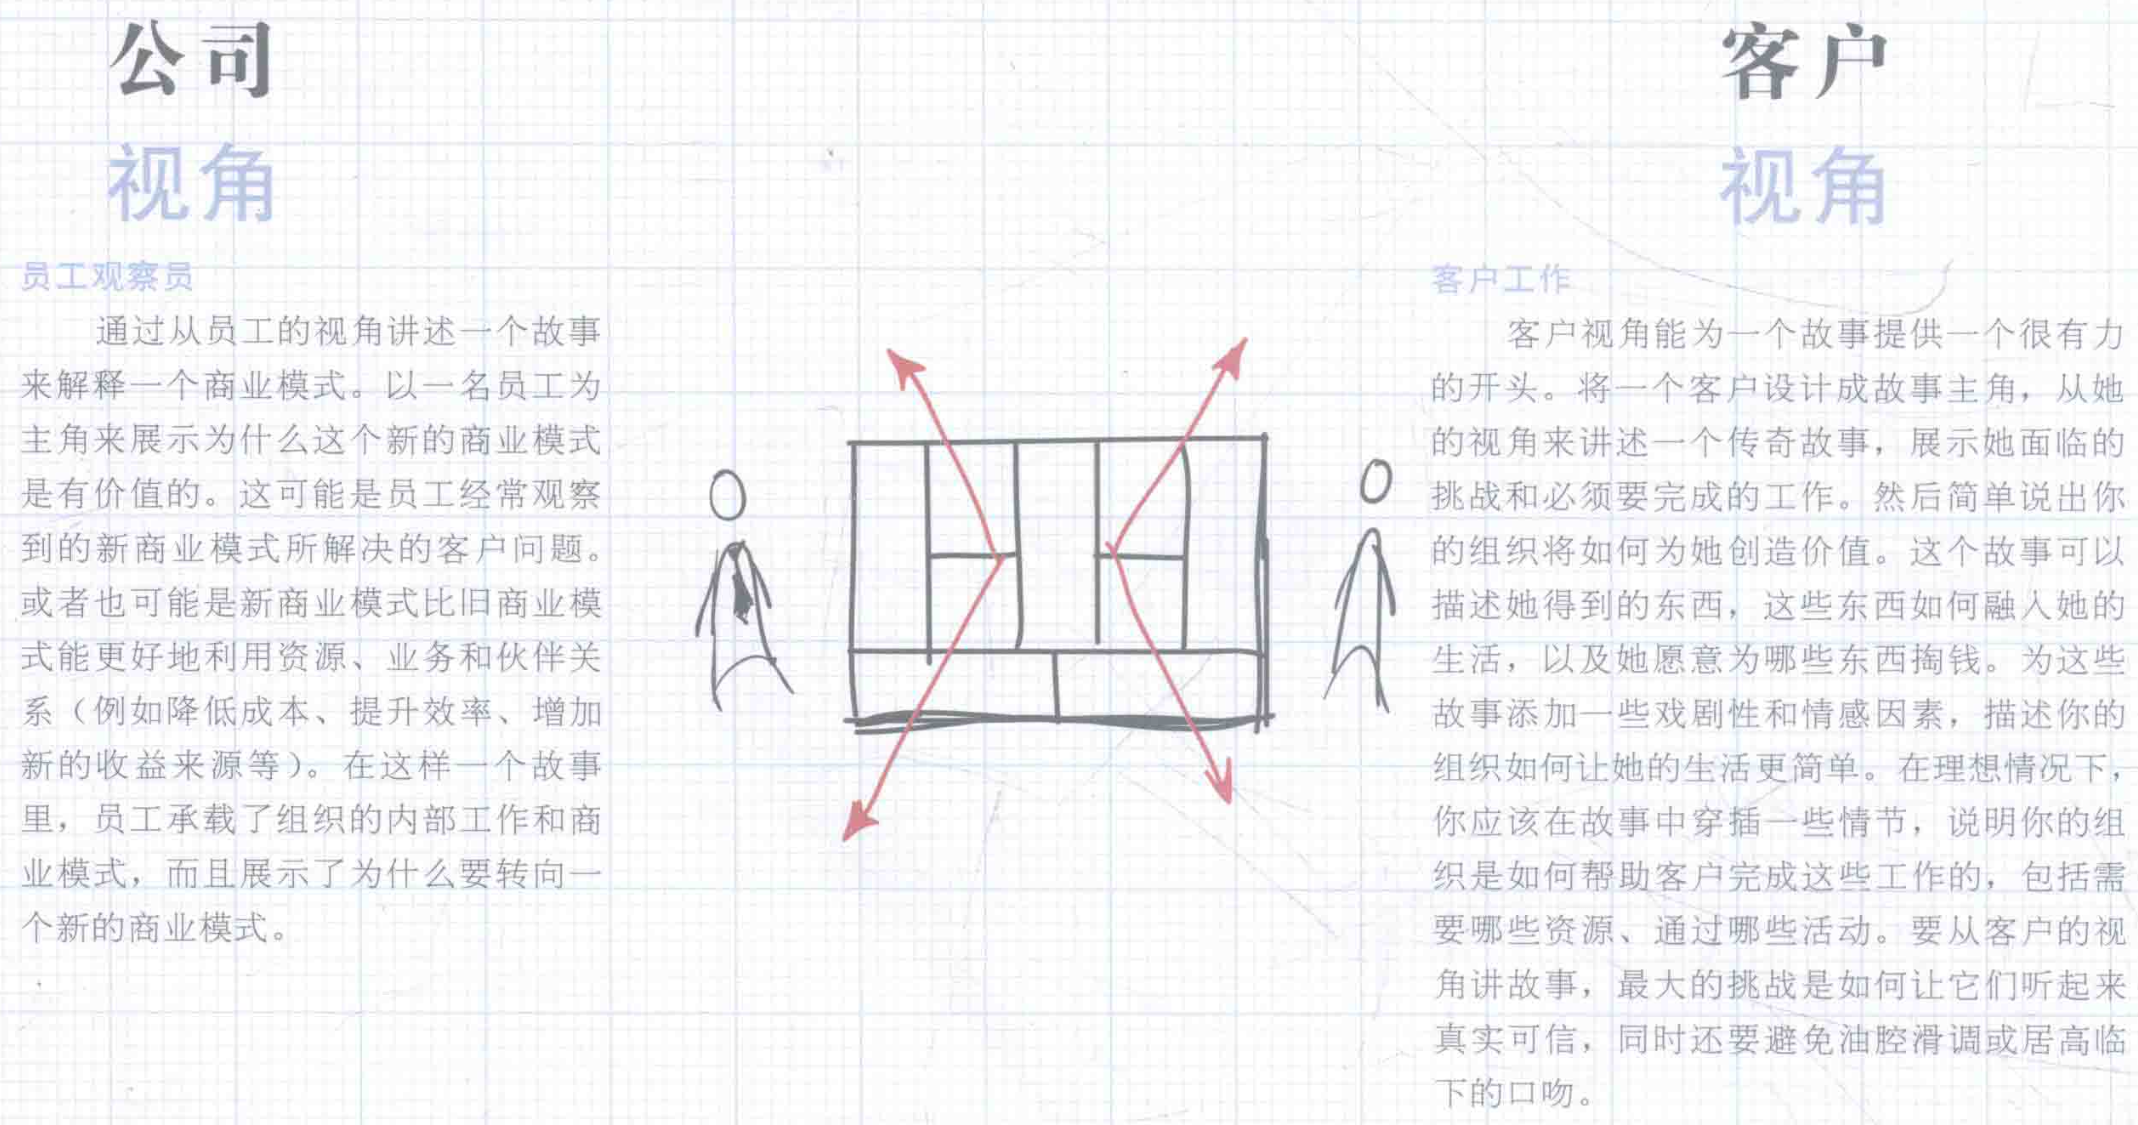
\includegraphics[width=0.7\textwidth]{img/故事的不同视角.png}
    \vspace{-0.5em}
\end{figure}

\subsubsection{讲故事的方法}

\begin{table}[H]
    \centering
    \resizebox{\textwidth}{!}{
        \begin{tabular}{|l|l|l|l|l|l|}
            \hline
                  & 图片和旁白                                                                  & 视频                                                                                & 角色扮演                                                                & 文字和图片                                                                   & 连环图画                                                                   \\ \hline
            描述    & \begin{tabular}[c]{@{}l@{}}用一张或很多张图片来\\ 讲述一个主角的故事和\\ 他的环境\end{tabular} & \begin{tabular}[c]{@{}l@{}}用视频来讲述一个主角\\ 的故事和他的环境可以\\ 拉近现实与幻想之间的\\ 距离\end{tabular} & \begin{tabular}[c]{@{}l@{}}让人们扮演故事中的主\\ 角,构建逼真形象的场\\ 景\end{tabular} & \begin{tabular}[c]{@{}l@{}}用文字和一到数张图片\\ 来讲述一个主角的故事\\ 及他的环境\end{tabular} & \begin{tabular}[c]{@{}l@{}}用一系列的卡通图片来\\ 栩栩如生地讲述一个主\\ 角的故事\end{tabular} \\ \hline
            何时用?  & 小组讨论或会场讲演                                                              & \begin{tabular}[c]{@{}l@{}}向一大群听众广播或者\\ 内部做有重要财务意义\\ 的决策\end{tabular}             & \begin{tabular}[c]{@{}l@{}}相互陈述新开发的商业\\ 模式创意的研讨会\end{tabular}       & \begin{tabular}[c]{@{}l@{}}向一大群听众汇报或广\\ 播\end{tabular}                  & \begin{tabular}[c]{@{}l@{}}向一大群听众汇报或广\\ 播\end{tabular}                 \\ \hline
            时间和成本 & 低                                                                      & 中/高                                                                               & 低                                                                   & 低                                                                       & 低/中                                                                    \\ \hline
            \end{tabular}
    }
    \end{table}


\subsection{场景}

场景能够很好地指导新商业模式的设计或者对当前商业模式的创新。场景也能让抽象的事物变得具体。
\begin{itemize}
    \item 不同的客户结构:产品或服务将被如何使用,什么样的客户会用到它们,客户的担忧、诉求和目标。
    \begin{itemize}
        \item 这些场景是基于客户洞察,但通过融入我们对客户的理解描绘出了独特、具体的图景。
        \item 通过描述具体的环境,客户场景能将客户洞察变得栩栩如生。
    \end{itemize}
    \item 商业模式未来可能的竞争环境:这里的目的不是为了预测未来,而是为了想象未来可能的具体细节。
    \begin{itemize}
        \item 这样能让创新者仔细体会未来各种环境下最合适的商业模式。
        \item 将场景规划的方法用到商业模式创新领域能让人品味到特定条件下商业模式会如何演进。
        \item 这能加深对商业模式及其必要调整措施的理解。更重要的是,它能够帮助我们对未来做好准备。
    \end{itemize}
\end{itemize}

将场景融入商业模式创新活动
\begin{figure}[H]
	\centering
	\vspace{-0.5em}
	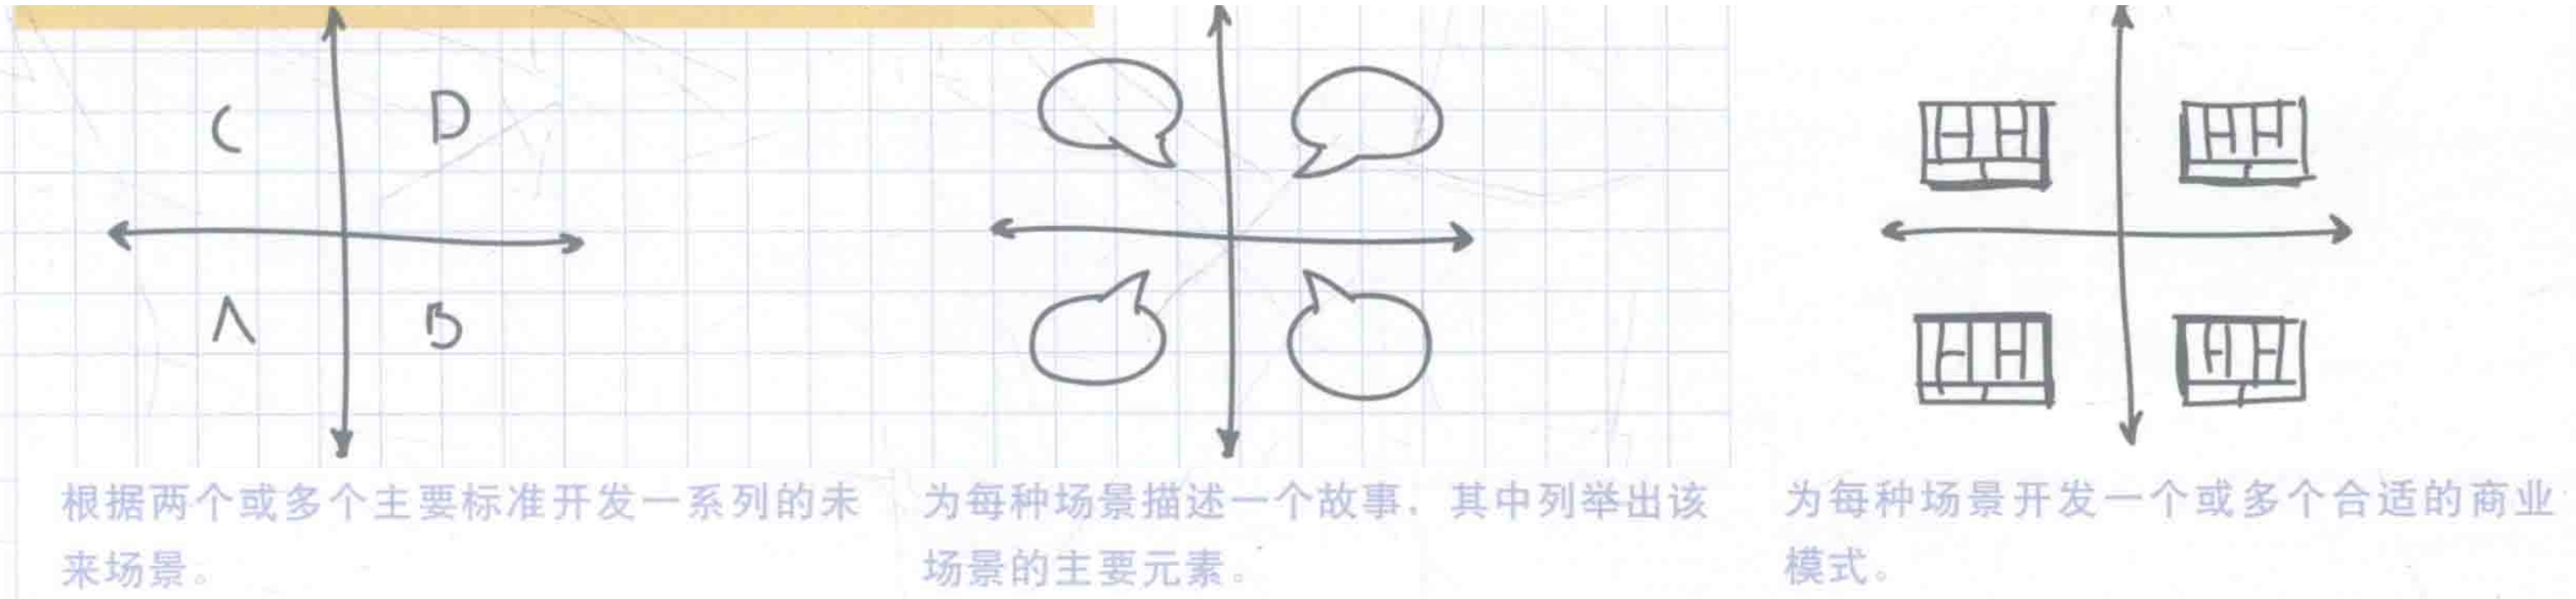
\includegraphics[width=0.8\textwidth]{img/将场景融入商业模式创新活动.png}
    \vspace{-0.5em}
\end{figure}

例:未来的医药商业模式
\begin{figure}[H]
	\centering
	\vspace{-0.5em}
	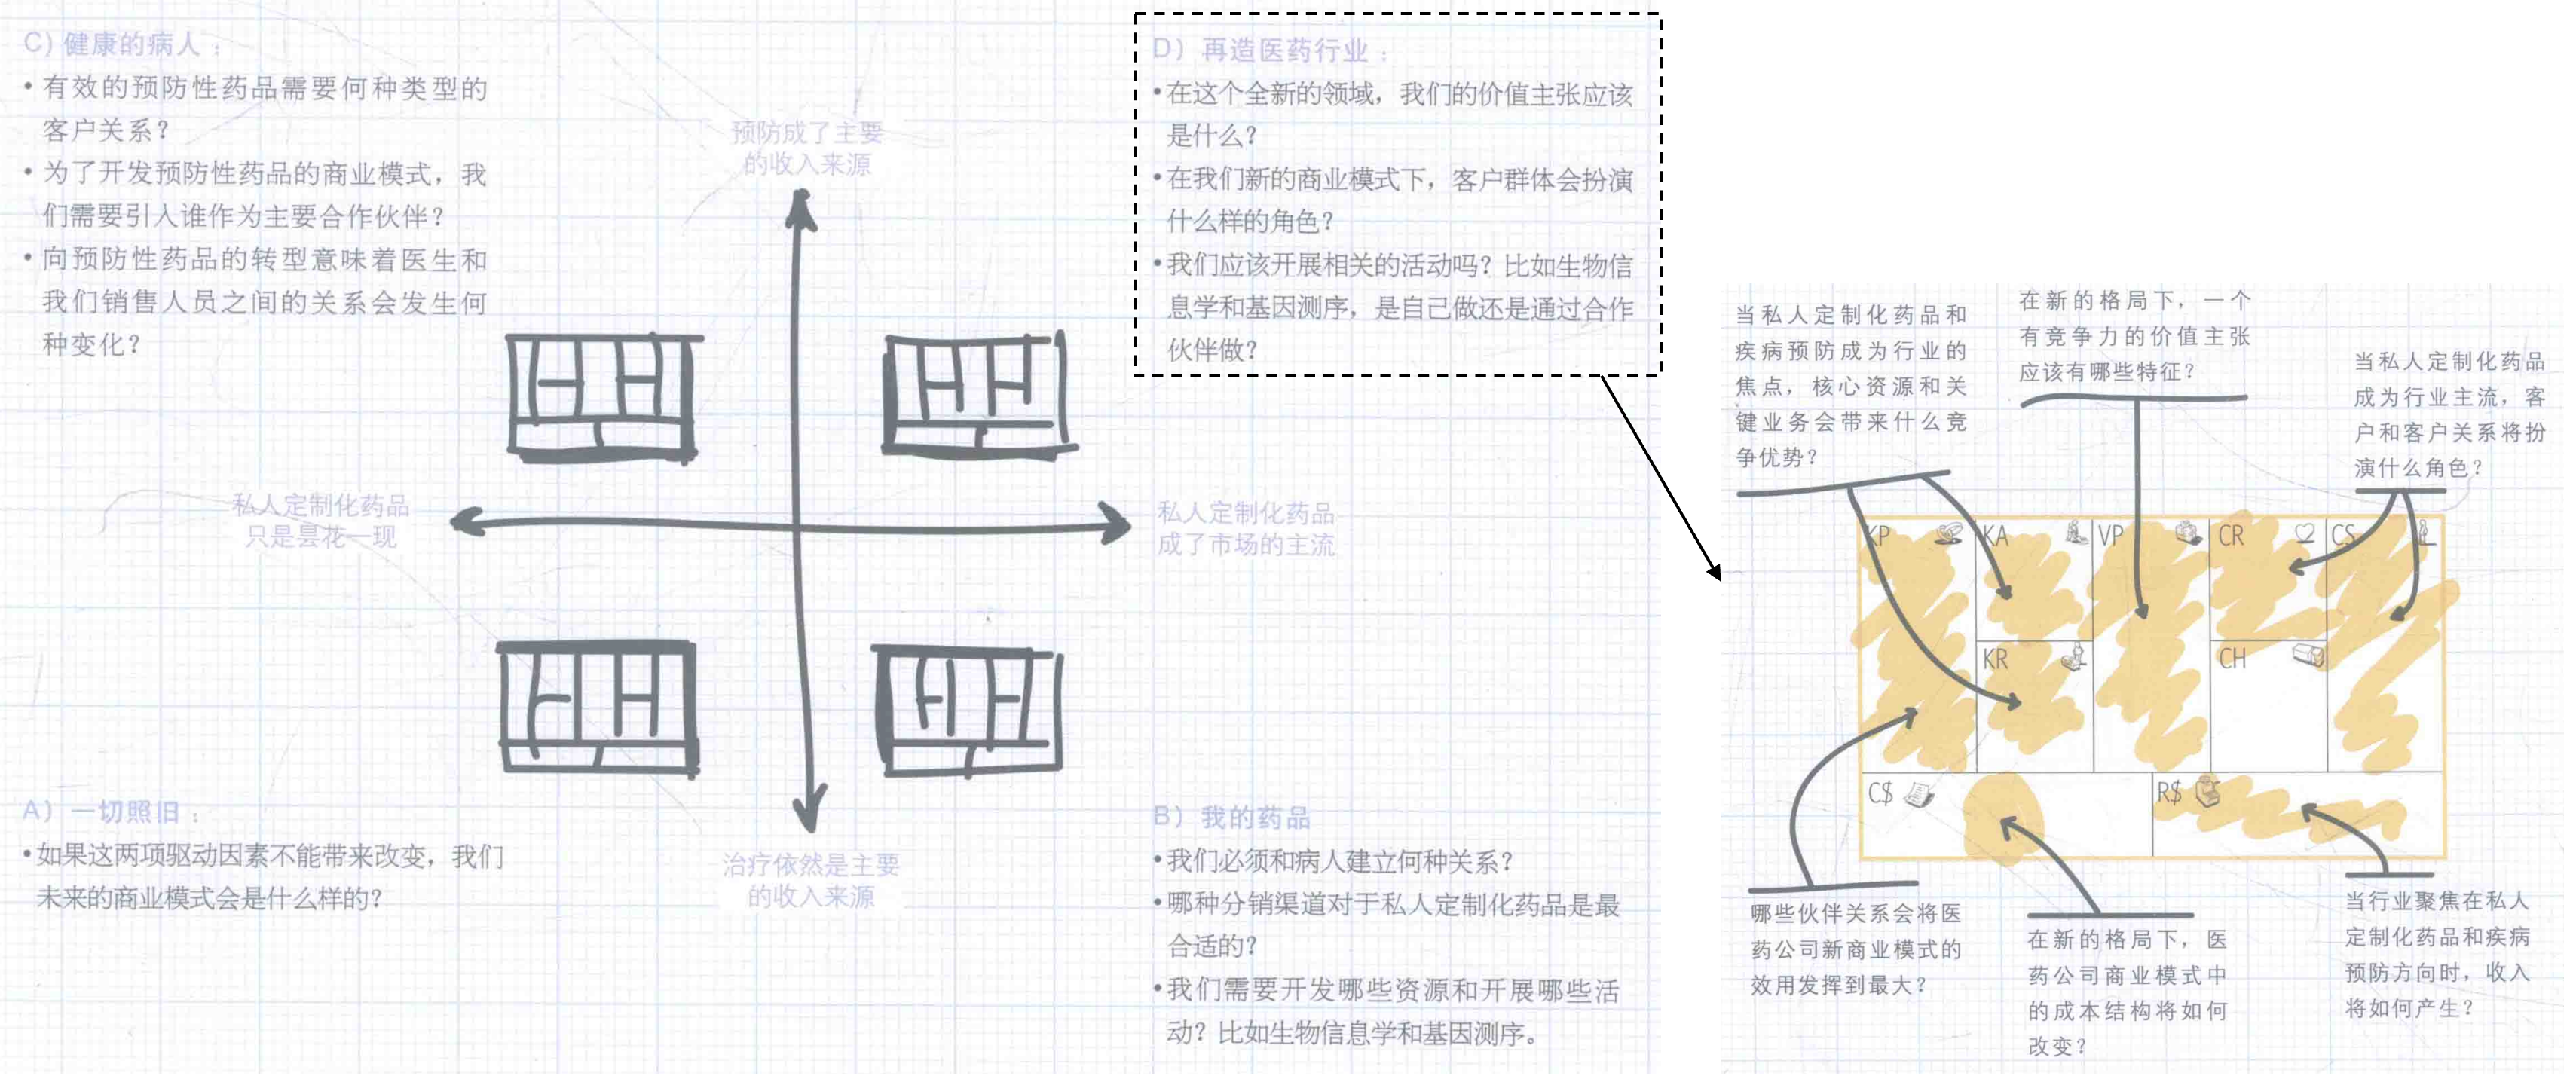
\includegraphics[width=\textwidth]{img/未来的医药商业模式.png}
    \vspace{-0.5em}
\end{figure}


